% !TEX root = ../../thesis.tex

\chapter{Introduction}
\label{ch:introduction}

\dictum[Alex Millane]{%
  I'm drinking a gin and tonic, without gin}%
\vskip 1em

A building, in its original manifestation, is a shelter. A means to protect the human body from harsh external conditions. And within this we ascribe the notion of the envelope, the barrier between the external and internal environments. It is the barrier that protects us from frigid temperatures, shades us from solar rays, and keeps us dry when a storm passes by. And over time, we have not just developed the quality of our envelopes, but also technologies that enable us to manufacture interior environments. The combination of heating, cooling, lighting and air handling enables us to exclude the energies of the exterior and form hermatic envelopes. Buildings transformed from mere shelters, to places of comfort where we now spend 87\% of our lives \cite{klepeis2001national}. We have in essence, become an indoor species. \

Unfortunately, the manufacture of interior environments comes with a large environmental impact. Buildings are currently responsible for 32\% of our final energy use and 19\% of our total greenhouse gas emissions \cite{IPCC}. There is, however, a 50\% - 90\% emission reduction potential using existing technologies \cite{IPCC}. On one hand, the efficiency of our manufactured interior environment can be increased. We can install more efficient systems to manufacture this energy at a lower environmental cost. We can further increase the isolation properties of our envelopes, thus reducing the energetic loss to the exterior. On the other hand, we can rewind the clock of architectural history and move back to a time where we did not manufacture internal environments, but rather mediated the external energies to fulfil that of the interior. These strategies, commonly described as passive design strategies, include aspects such as natural ventilation, thermal storage, and static shading. 

Instead of rewinding the clock of architectural history, there is also the possibility to look ahead. With new technologies the mediation of the external environment is not restricted to passive strategies, but also active ones. The mediation of solar radiation through responsive shading is one such example. A responsive shading system will open when solar radiation levels are low to maximise natural lighting, and close when the radiation reaches a critical peak at which the building begins to overheat. Iconic examples include the Al Bahr Towers in Dubai \cite{oborn2012bahr}, the Arab World Institute in Paris, and the ThyssenKrupp Headquarters in Essen. 

%These responsive envelopes are beneficial in reducing overall energy consumption, but lacks flexibility as the designer must set the threshold radiation levels at which the envelope opens and closes

In an ideal setting, as shown in Figure \ref{fig:facadefunctions}, the envelope does not just exist in an open or closed state, but in a multitude of states fullfilling various functions. The modularity described in this schematic enables certain parts of the envelope to respond for optimal daylight distribution, whereas others are optimised for heating / cooling demand reduction, and enhancing views to the exterior. If we also replace the envelope material with light weight thin film solar panels, we can also harvest solar energy onsite and use it to meet the demands of the interior space. It is through this modularity that we can best balance user comfort, with building energy saving.

This modularity however introduces new challenges in terms of control. In a responsive system the designer sets threshold radiation levels at which the envelope opens and closes. This modular envelope however, can have thousands of possible states, and needs to find the optimum balance between building energy demand reduction, occupant comfort, and PV electricity production. It is in this context that we coin the term adaptive. An adaptive envelope senses it's environment, such as the occupancy, interior temperature, exterior temperature and radiation levels, and then determines the optimum envelope configuration to mediate a comfortable interior environment while minimising the total net energy consumption. 

This adaptive nature can span different time durations. In the short time span, if the sun goes behind a cloud, or the occupancy dramatically increases, the envelope will be able to adapt to meet this new environment. Likewise, the envelope will also adapt to long term variations such as global warming. 

This dissertation is written in the context of the Adaptive Solar Facade (ASF), an adaptive photovoltaic envelope designed for a research and innovation unit known as the HiLo \cite{Block2017}. The ASF is a modular facade of 40 x 40 cm copper indium galium selenide (CIGS) PV panels that can be actuated in two degrees of freedom with a range of 90$^{\circ}$. An example of this, mounted on a testing site can be seen in Figure \ref{fig:ASFNest}.


\begin{figure}
\begin{center}
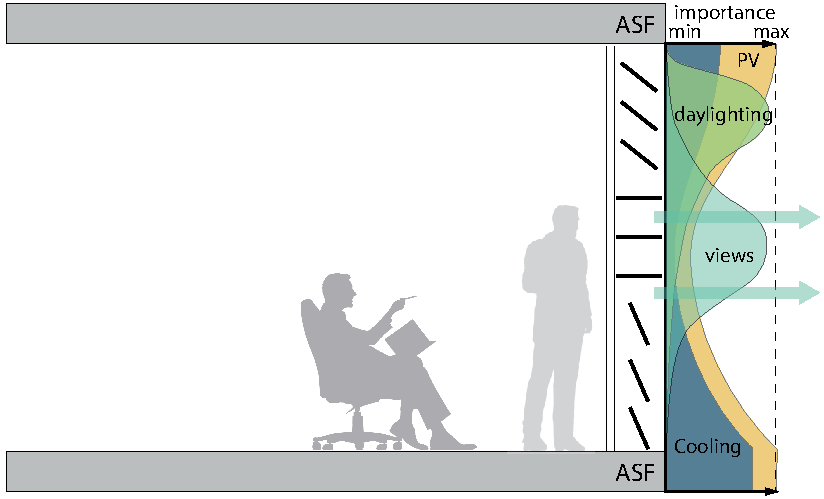
\includegraphics[width=\columnwidth, trim= 0cm 0cm 0cm 0cm,clip]{\dir/facadeFunctionsnew.pdf}
\caption{A modular facade adpative to various functions for optimising occupant comfort}
\label{fig:facadefunctions}
\end{center}
\end{figure}

\begin{figure}
\begin{center}
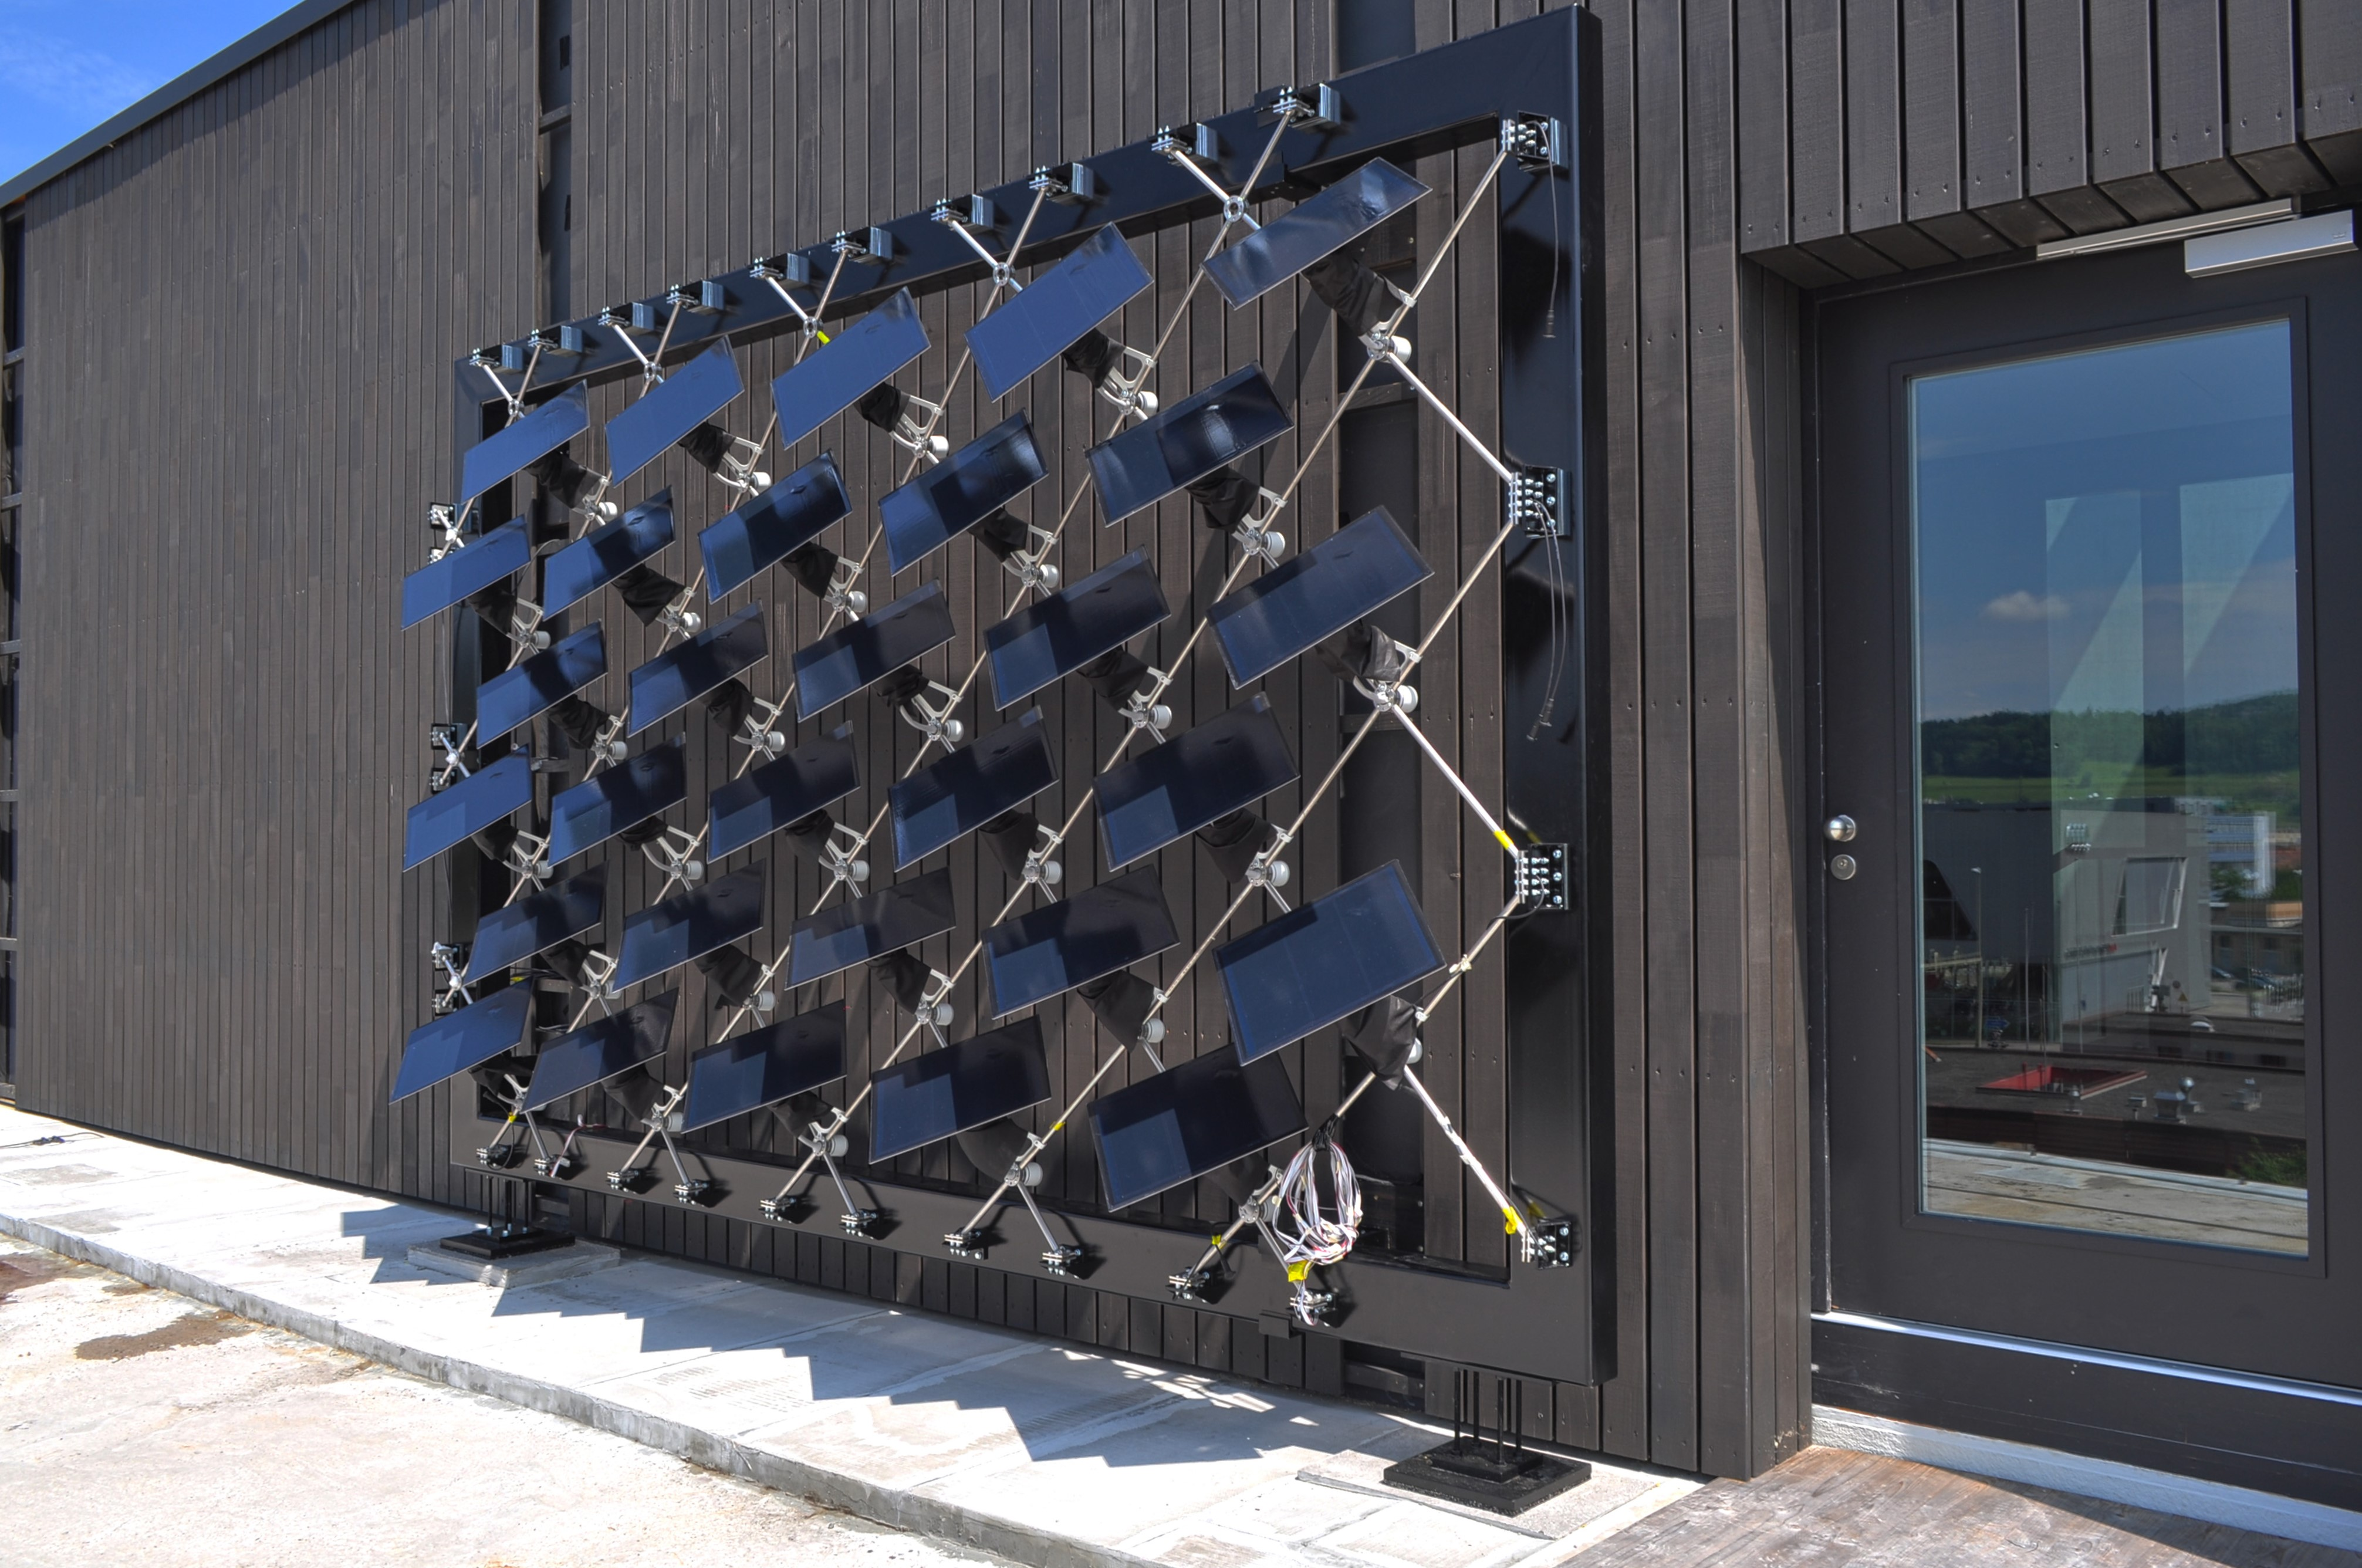
\includegraphics[width=\columnwidth, trim= 0cm 0cm 0cm 0cm,clip]{\dir/ASFNest.JPG}
\caption{The final Adaptive Solar Facade, mounted on a testing site prior to assembly on the HiLo Module}
\label{fig:ASFNest}
\end{center}
\end{figure}




\section{Research Questions}

The four questions addressed in this research are 

\begin{itemize}
\item How can complex architectural components, such as the ASF be designed and constructed? 
\item How can a photovoltaic envelope be controlled to be adaptive?
\item What is the energy saving potential of an adaptive photovoltaic envelope?
\item How does the energy saving potential vary for different building types?
\item What is the life cycle CO$_2$ saving potential of an adaptive photovoltaic facade?

\end{itemize}

\section{Organisation of the Thesis}

The remainder of this thesis is composed of three journal papers and one conference paper. Chapter \ref{ch:asfDesign} introduces the parametric design environment, which was created for rapid iterative development of the ASF. This chapter also introduces some of the design elements of the ASF. Chapter \ref{ch:asfSimulation} introduces the model predictive control strategy to allows for adaptive control. This chapter first introduces the simulation methodology, and then discusses the energy saving potential of an ASF system. Chapter \ref{ch:asfArchetype} takes on the model from Chapter \ref{ch:asfSimulation} and runs an evaluation on eleven different building use types spanning six construction periods. Chapter \ref{ch:asfLCA} then takes the results of the energy simulation methodology and assesses the carbon life cycle cost. Finally Chapter \ref{ch:conclusion} concludes the thesis. 